\newpage
\chapter{Introduction}
\label{chap:introduction}

\ac{U-SPACE} is a student project at the Rymdcampus of the \ac{LTU} in Kiruna under the supervision of Kjell Lundin (\ac{IRF}) and Alf Wikström (\ac{LTU}). It is supported by \ac{IRF} and \ac{LTU}. The goal of this project is to prove the concept of a small-scale student-built unmanned \ac{SPA}. The solar cells that power the airship are mounted on a gas-filled envelope, with forward propulsion being achieved by propellers mounted onto the same envelope. The airship communicates via two separate wireless connections with a controller and a ground station. These communication channels enable human control over the airship, together with the retrieval of housekeeping and scientific payload data. The payload data consists of measurements from several sensors (magnetometer, accelerometer, gyroscope and \ac{GPS}) and images collected by a small on-board camera. On the ground station, the image data and the sensor data are combined to construct an aerial map of the flight environment.
\\
\\
The concept of a \ac{SPA} has attracted major interest in recent years \cite{website:ravenaerostar, website:gaya, poster:saba, report:colozza2004, website:solr, website:ISIS, website:helios, website:solarship, website:knarr}. Applications for this type of airship reach far and wide, ranging from passenger and cargo transport \cite{website:gaya, website:solr, website:helios, website:solarship, website:knarr} over scientific research \cite{poster:saba} and surveillance \cite{website:ravenaerostar, website:ISIS, website:helios} to planetary exploration \cite{report:colozza2004}. In Scandinavia there have been several studies on using airships for the transport of windmill structures \cite{website:knarr, website:energimyndigheten} and the windmill company Vestas has filed a patent on this method \cite{website:vestas}. The actual implementation of the \ac{SPA} concept varies greatly. Solar Ship \cite{website:solarship} is a hybrid of an aircraft and an airship, while Project Sol'r \cite{website:solr} has the intention of building a manned \ac{SPA}, in contrast to many of the other implementations. Some airships are intended for low-altitude flight \cite{website:solr, website:helios}, while other airships are meant to fly at 18 km altitude or above \cite{website:ravenaerostar, poster:saba, website:ISIS}. Regardless of their exact implementation or application all \ac{SPA}s benefit greatly from the advantages of this concept: simple flight control, reduced fossil fuel consumption and access to long duration flights. Apart from these inherent strong points, other advantages of \ac{SPA}s are the possibility for autonomous take-off and landing, the elimination of large infrastructures like airports, reduced weather constraints and relatively low costs \cite{website:ravenaerostar, website:gaya}.
\\
\\
Even though many research groups and commercial companies have investigated the possibilities of \ac{SPA}s, very few student-driven projects exist. Projet Sol'r \cite{website:solr} for example, created by a team of French students, has the intention of piloting a \ac{SPA} across the English Channel. This team is the exception in all projects discussed previously. The above-mentioned advantages of \ac{SPA}s and the fact that few student projects exist, were the main drivers for the creation of the \ac{U-SPACE} project at \ac{LTU}.

\section{Hardware}
\label{sec:intro_hardware}

The hardware for the \ac{U-SPACE} project can be divided into four subsystems, as visualized in the block diagram of Figure \ref{fig:hardware_block}. This hardware is present both in the airborne structure (the \ac{SPA}) and in the ground-based part of the project (the ground station and controller).

\begin{figure}[htbp!]
\centering
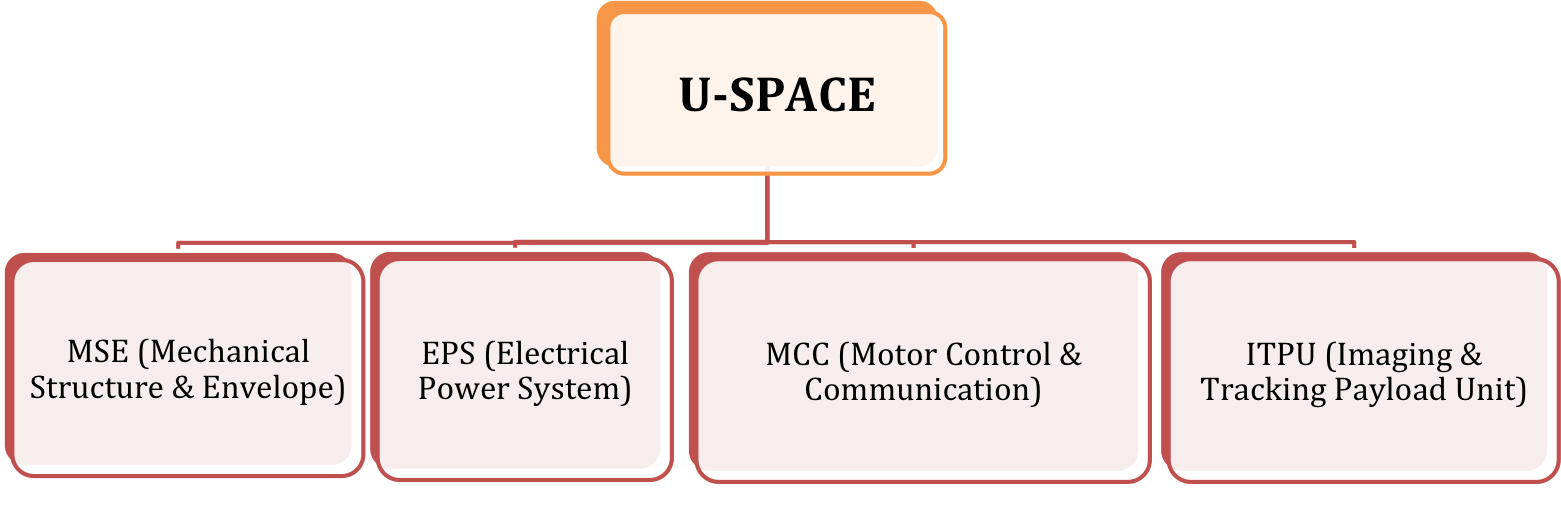
\includegraphics[width=\textwidth]{figures/hardware_block.png}
\caption{Hardware block diagram of the U-SPACE project}
\label{fig:hardware_block}
\end{figure}

\subsection{On-board Hardware}

The first subsystem is the \ac{MSE}. This subsystem is the principal mechanical structure of the airship. It includes a gas-filled envelope, a payload bay and structures to mount both the solar cells and the propellers. This subsystem is the support for all other subsystems and provides the lift to allow the \ac{SPA} to fly. More information can be found in chapter \ref{chap:mse}. The second subsystem, the \ac{EPS}, is responsible for generating solar power, distributing this power to all other subsystems and storing the generated energy when required. It makes use the \ac{MSE} subsystem which supports the solar cells, while it also allows both forward propulsion and the generation of scientific payload data.  Chapter \ref{chap:eps} provides the details on this subsystem. The third subsystem, \ac{MCC}, takes care of the forward propulsion of the airship by employing propellers mounted onto motors. The structural link to the airship is the responsibility of the \ac{MSE}, while power is provided by the \ac{EPS}. The motors are controlled via a wireless connection, which is also the responsibility of this subsystem. A more thorough discussion can be found in chapter \ref{chap:mcc}. The final subsystem, the \ac{ITPU}, is the scientific payload of the \ac{SPA}. It consists of several different sensors (including a magnetometer, an accelerometer, a gyroscope and a \ac{GPS}) mounted inside the payload bay (part of the \ac{MSE}). The data from these sensors is processed with the help of a \ac{MCU}. The payload bay also contains a camera which can take pictures from the ground that are saved on board or transmitted to a ground station via a second wireless connection. The sensor data is also sent to the ground station via this wireless connection. The power for the sensors, the \ac{MCU}, the camera and the wireless connection is provided by the \ac{EPS}. Chapter \ref{chap:itpu} discusses this subsystem in more detail.

\subsection{Ground-based Hardware}

The hardware for the ground station and for the wireless control are respectively part of the \ac{ITPU} and \ac{MCC} subsystems (see chapters \ref{chap:itpu} and \ref{chap:mcc} respectively).  This hardware consists of a receiver for the scientific payload data and a transmitter/receiver for the control of the \ac{SPA}.  In order to present the scientific payload data from the sensors and the camera, a means to visualize this \ac{ITPU} data is required as well.

\section{Software}
\label{sec:intro_software}

\enlargethispage{2.0em}

The software required for the \ac{U-SPACE} project is only present in the on-board \ac{ITPU} subsystem and in the ground station used to receive the scientific payload data from this subsystem. The other subsystems do not require the development of any software. A block diagram of the software is presented in Figure \ref{fig:software_block}.

\begin{figure}[h!]
\centering
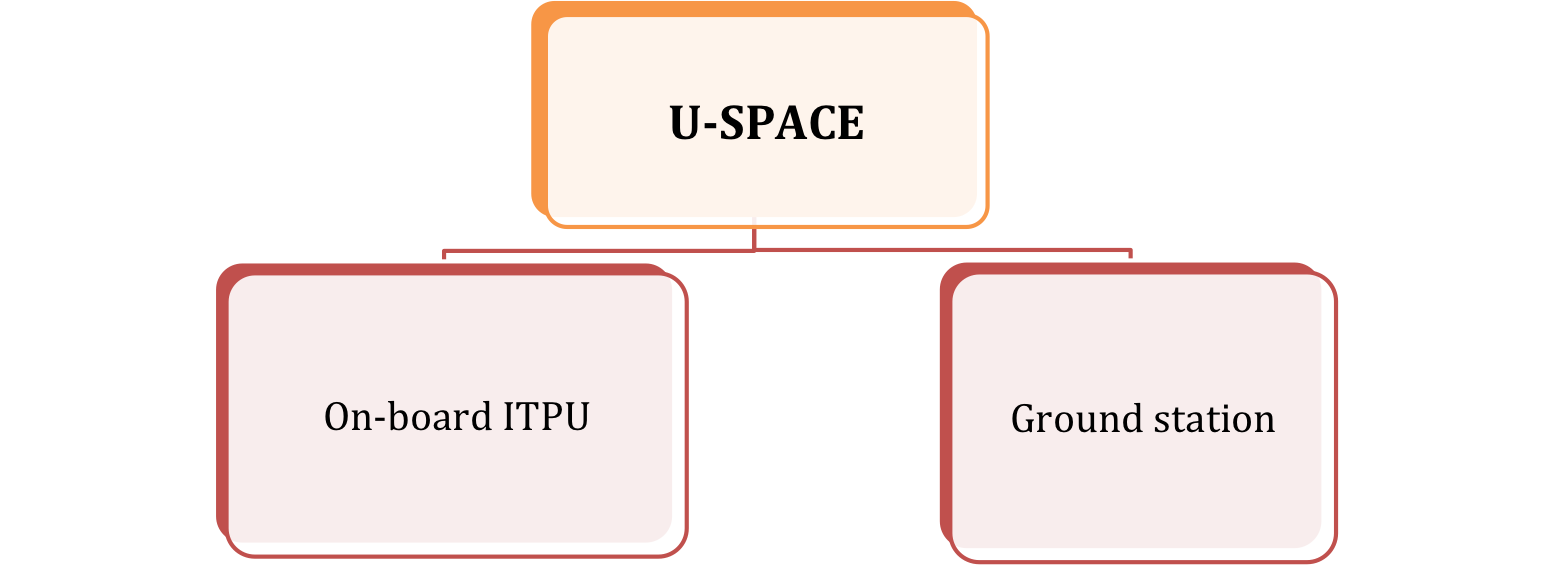
\includegraphics[width=\textwidth]{figures/software_block.png}
\caption{Software block diagram of the U-SPACE project}
\label{fig:software_block}
\end{figure}

\subsection{On-board Software}

The software on board the \ac{SPA} reads the data from the sensors (magnetometer, accelerometer, gyroscope and \ac{GPS}) and fuses this data in order to obtain more accurate information about the orientation and position of the airship. The software is also responsible for sending this scientific payload data to the ground station via the dedicated wireless connection. Finally the on-board software is needed to control the camera and to take pictures from the ground below the airship. The pictures are saved on board or sent to the ground station via a wireless connection. A description of this software can be found in chapter \ref{chap:itpu}.

\subsection{Ground-based Software}

The ground station also requires the development of some software. This software is mainly responsible for receiving sensor data from the airship via the wireless connection, but it is also needed for the visualization of this data. It runs an algorithm that combines the data from the sensors and the images taken by the camera in order to obtain a complete aerial map of the landscape over which the \ac{SPA} is flying. Once again chapter \ref{chap:itpu} provides more details.

\subsection{Operational Modes}

With the development of the on-board and ground-based software modules, several operational modes related to the scientific payload become possible in the \ac{U-SPACE} project. The basic modes are listed below:

\begin{enumerate}
\item Read out data from sensors and fuse the data
\item Control the camera to take pictures from the ground
\item Combination of mode 1 and mode 2
\end{enumerate}